f\section{Theorie}
In diesem Versuch werden mithilfe eines Germaniumdetektors die Spektren
unterschiedlicher radioaktiver Quellen untersucht. Anhand dieser Daten sollen unter Anderem
die Aktivität einer Quelle errechnet werde oder die Zusammensetzung eines unbekannten Objektes bestimmt 
werden. 

Im Allgemeinen wird radioaktive Strahlung durch ihre Art der Entstehung und Reichweite unterschieden. 
Dabei handelt es sich um $\alpha$-, $\beta$- und $\gamma$-Strahlung. In diesem Versuch wird $\gamma$-Strahlung
untersucht. Diese Art von ioniserender Strahlung entsteht beim Zerfall von Atomkernen, die sich nach einem $\alpha$- oder 
$\beta$-Zerfall im angeregten Zustand befinden. Beim Übergang von dem angeregten Zustand in den Grundzustand oder einen
weniger angeregten Zustand wird Energie in Form eines $\gamma$-Quants frei. Da es sich bei dem $\gamma$-Quant um ein 
ungeladenes Teilchen handelt wechselwirkt es deutlich weniger als beispielsweise die $\alpha$-Strahlung. Somit weist die 
$\gamma$-Strahlung die höchste Durchdringungskraft von Materie auf. \\
Je nach Energie wechselwirken die $\gamma$-Quanten dennoch mit der umliegenden Materie. 
Die Abhängigkeit der Wechselwirkungsart von der Photonenernergie ist in abbildung \ref{fig:WW}
dargestellt.
\begin{figure}[H]
    \centering
    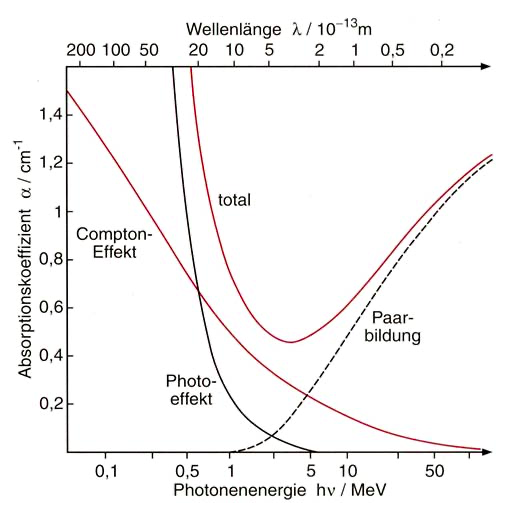
\includegraphics[width=0.8\textwidth]{WW.png}
    \caption{Energieabhängigkeit der Wechselwirkungsarten von Photonen mit Materie \cite{WW}.}
    \label{fig:WW}
\end{figure} \noindent
Wie in Abbildung \ref{fig:WW} zu erkennen ist, ist bei kleinen Energien der Photoeffekt der 
dominate Wechselwirkungsprozess. Dabei sind eingetrahlte Photonen in der Lage Elektronen aus 
einem Metall zu lösen, wenn ihre Energie groß genug ist die materialspezifische Austrittsabeit
zu überwinden. Typische Austrittsarbeitenn liegen im Bereich von einigen Elektronenvolt. So beträgt 
die Austritssarbeit bei Caesium beispielsweise $\SI{1,94}{\electronvolt}$ und bei Germanium
ca. $\SI{5}{\electronvolt}$. Die Energie der Photonen, die über die Austrittsarbeit hinausgeht
führen die herausgelösten Elektronen in Form von kinetischer Energie 
\begin{equation}
    E_\text{kin} = E_\text{Photon} - W_\text{Austritt}
\end{equation}
mit sich. Durch das Herauslösen des Elektrons bleibt ein Loch zurück, welches durch ein Elektron 
aus einer höheren Schale gefüllt wird. Dabei wird Energie in Form von Röntgenstrahlung frei, die 
jedoch im Absorber verbleibt. \\ 
In einem Energiebereich von ca.$\SI{100}{\kilo\electronvolt}$ bis $\SI{10}{\mega\electronvolt}$ dominiert
der Comptoneffekt. Beim Comptoneffekt wird das Photon an einem ruhenden Teilchen getreut. 
Durch die Streuung kommt es zu einem Energieverlust und damit zu einer Vergrößerung der 
Wellenlänge. Die Änderung der Wellenlänge ist dabei abhängig vom Streuwinkel zwischen Photon und 
Elektron. Die Wahrscheinlichkeit für das Auftreten der Compton-Streuung wird durch den 
Klein-Nishina-Wirkungsquerschnitt angegeben. Dieser gibt dabei die Wikelverteilung der getreuten
Photonen an. 
Der differentielle Wirkungsquerschnitt in Abhängigkeit der Energie ist durch
\begin{equation}
    \frac{d\sigma}{d\Omega} = \frac{1}{2} \frac{\alpha^2}{m^2} \left(\frac{E'}{E}\right)^2 \left[\frac{E'}{E}+\frac{E}{E'}-\sin(\theta)^2\right]
\end{equation} \noindent
gegeben. Wobei E' der Energie des gestreuten und E der Energie des eingestrahlten Photons entspricht.